\documentclass[a4paper]{article}
\usepackage[spanish]{babel}
\usepackage[utf8]{inputenc}
\usepackage{graphicx}
\usepackage{enumerate}
\usepackage{listings}
\usepackage{color}
\usepackage{indentfirst}
\usepackage{fancyhdr}
\usepackage{latexsym}
\usepackage[colorlinks=true, linkcolor=black]{hyperref}
%\usepackage{makeidx}
%\usepackage{float}
\usepackage{calc}
\usepackage{amsmath, amsthm, amssymb}
\usepackage{amsfonts}
%\lstset{language=C}
\definecolor{gray}{gray}{0.5}
\definecolor{light-gray}{gray}{0.95}
\definecolor{orange}{rgb}{1,0.5,0}

\usepackage{fancyhdr}
\pagestyle{fancy}

%\renewcommand{\chaptermark}[1]{\markboth{#1}{}}
\renewcommand{\sectionmark}[1]{\markright{\thesection\ - #1}}

\fancyhf{}

\fancyhead[LO]{Sección \rightmark} % \thesection\ 
\fancyfoot[LO]{\small{Yanet Giuseppin, Laura Muiño, Javier San Miguel, Axel Straminsky}}
\fancyfoot[RO]{\thepage}
\renewcommand{\headrulewidth}{0.5pt}
\renewcommand{\footrulewidth}{0.5pt}
\setlength{\hoffset}{-0.8in}
\setlength{\textwidth}{16cm}
%\setlength{\hoffset}{-1.1cm}
%\setlength{\textwidth}{16cm}
\setlength{\headsep}{0.5cm}
\setlength{\textheight}{25cm}
\setlength{\voffset}{-0.7in}
\setlength{\headwidth}{\textwidth}
\setlength{\headheight}{13.1pt}

\renewcommand{\baselinestretch}{1.1}  % line spacing


% \setcounter{secnumdepth}{2}
\usepackage{underscore}
\usepackage{caratula}
\usepackage{url}
\usepackage{float}

\newcommand{\cod}[1]{{\tt #1}}
\newcommand{\negro}[1]{{\bf #1}}
\newcommand{\ital}[1]{{\em #1}}
\newcommand{\may}[1]{{\sc #1}}
\newcommand{\tab}{\hspace*{2em}}

\hypersetup{
 pdfstartview= {FitH \hypercalcbp{\paperheight-\topmargin-1in-\headheight}},
 pdfauthor={Grupo},
 pdfsubject={Dise\~{n}o}
}

\lstdefinestyle{customc}{
  backgroundcolor=\color{light-gray},
  belowcaptionskip=1\baselineskip,
  breaklines=true,
  numbers=left,
  xleftmargin=\parindent,
  language=C,
  showstringspaces=false,
  basicstyle=\footnotesize\ttfamily,
  keywordstyle=\bfseries\color{blue},
  commentstyle=\itshape\color{gray},
  identifierstyle=\color{black},
  stringstyle=\color{orange},
}

\lstdefinestyle{customasm}{
  backgroundcolor=\color{light-gray},
  belowcaptionskip=1\baselineskip,
  numbers=left,
  xleftmargin=\parindent,
  language=[x86masm]Assembler,
  keywordstyle=\bfseries\color{blue},
  basicstyle=\footnotesize\ttfamily,
  commentstyle=\itshape\color{gray},
}

\lstset{escapechar=@}


\begin{document}

\thispagestyle{empty}
\materia{Métodos Numéricos}
\submateria{Segundo Cuatrimestre de 2015}
\titulo{Trabajo Práctico I}
%\subtitulo{Scheduling}
\integrante{Yanet Giuseppin}{184/11}{yanetagiu@yahoo.com}
\integrante{Laura Muiño}{399/11}{mmuino@dc.uba.ar}
\integrante{Javier San Miguel}{786/10}{javiersm00@fmail.com}
\integrante{Axel Straminsky}{769/11}{axelstraminsky@gmail.com}

\makeatletter

\maketitle
\newpage

\thispagestyle{empty}
\vfill

\thispagestyle{empty}
\vspace{3cm}
\tableofcontents
\newpage

\newenvironment{myindentpar}[1]
{\begin{list}{1}
         {\setlength{\leftmargin}{#1}}
         \item[]
}
{\end{list} }

%\normalsize
\newpage

% -------------------------------------------------------
% Breve explicacion de la base teorica que fundamenta los metodos involucrados en el trabajo, junto con los metodos mismos.  
% -------------------------------------------------------
\section{Introducción Teórica}

\subsection{El Problema y su representación}
Queremos medir temperaturas de un horno industrial cilíndrico utilizado para fundir metales. Dicho horno tiene una pared interior y una exterior, cuyas temperaturas (la de las paredes) son conocidas en determinados puntos. Sabemos que la pared exterior tiene un límite de temperatura máxima, y nuestro objetivo es determinar si dicha temperatura máxima es alcanzada o no. Para ello, buscamos los puntos en el horno cuya temperatura alcance los 500 grados celcius.  Si esta temperatura es cercana al borde exterior se corre peligro por parte de los trabajadores de una hipotética fábrica que utilice dicho horno.


\begin{wrapfigure}{r}{0.5\textwidth}
  \vspace{-20pt}
  \begin{center}
    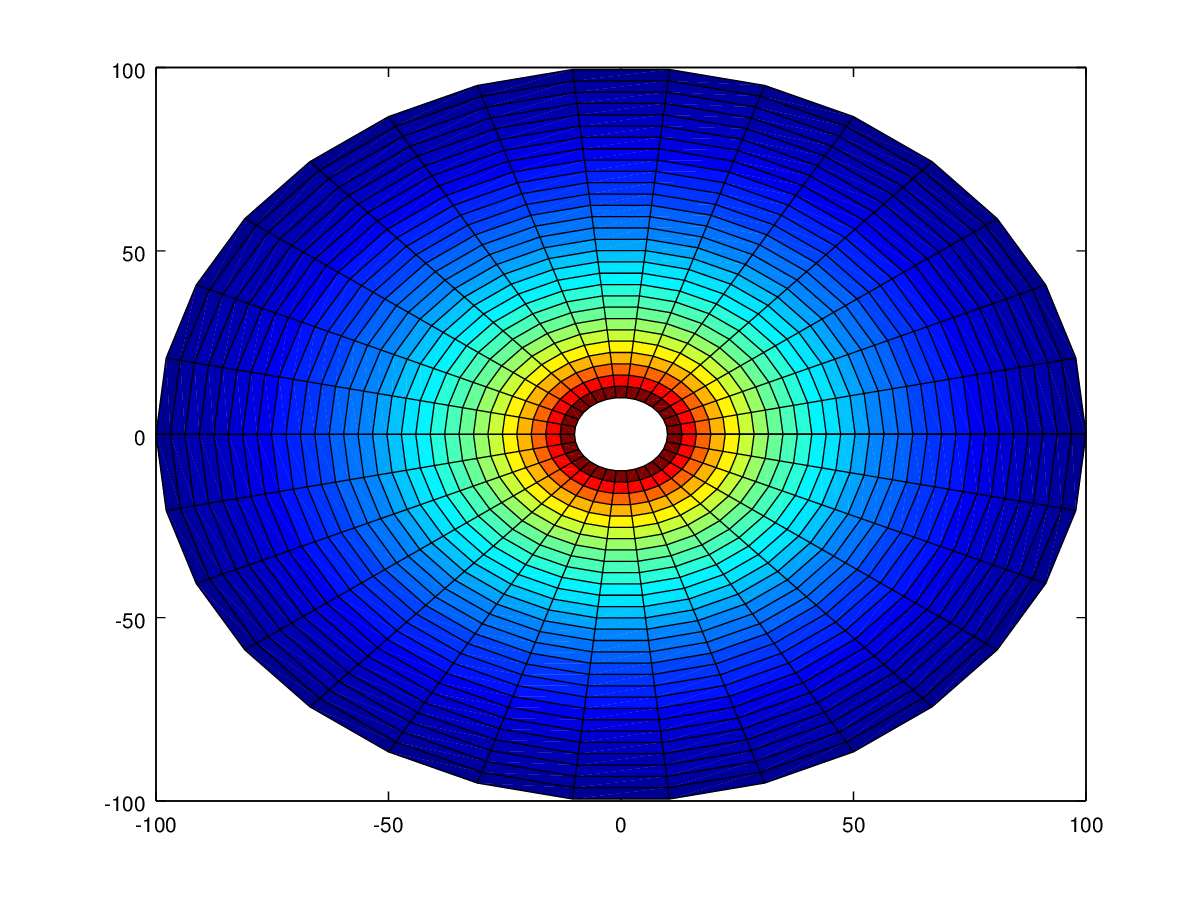
\includegraphics[scale= 0.4]{../hornoEjemplo.png}
  \end{center}
  \vspace{-20pt}
  \caption{Temperatura de un horno.}
  \vspace{-10pt}
  \label{fig:corteHorno}
\end{wrapfigure}


El problema se reduce a determinar dónde se encuentra la isoterma 500 en un círculo, como el que se ve en la figura, que representa un corte del horno. Las pared externa del horno es la circunferencia, y la pared interna es la circunferencia del circulo interno.



\subsection{Solucionando el problema}

Usando las herramientas aprendidas en la materia (sistemas de ecuaciones lineales, y sus métodos de solución, como Eliminación Gaussiana o factorización LU) queremos representar las temperaturas en distintos puntos del horno como incógnitas de un sistema lineal de ecuaciones que resolveremos.
 Para esto vamos a discretizar el espacio para tener finitas incógnitas, y vamos a usar ecuaciones de calor y la información de las temperaturas en finitos puntos de las paredes y así armar la matriz con los coeficientes del sistema.

 %explicar la discretizacion

 % explicar las ecuaciones de calor




A continuación hay una breve introducción a los algoritmos conocidos y teoría que aplicamos y usamos en el trabajo.

\subsubsection{Eliminación Gaussiana}
Dada una matriz A $\in R^{nxn}$ queremos resolver el sistema $Ax = b$. El algoritmo de Eliminación Gaussiana se usa para simplificar el sistema de ecuaciones ya que produce una matriz triangular superior equivalente a la original. Esto facilita el despeje de las incógnitas con el uso de otro algoritmo llamado Backward Substitution. Las tres operaciones principales que se llevan a cabo son, suma entre filas, multiplicación de una fila por un coeficiente distinto de cero e intercambio de filas. Dichas operaciones mantienen la equivalencia.

\subsubsection{Backward Substitution}
El método Backward Substitution consiste en la obtención de los valores de las incógnitas a partir de la matriz triangulada. El método recorre cada fila de esta matriz en orden decreciente en filas. Con lo que el despeje de las incógnitas simplemente consiste en despejar el valor de la diagonal respecto al resto de los valores ya obtenidos en iteraciones anteriores.

\subsubsection{Factorización LU}
El algoritmo de Factorización LU surge ante el problema que se presenta cuando queremos resolver un sistema de ecuaciones similar a uno anteriormente resuelto. Dado el sistema de ecuaciones $Ax = b$, una vez obtenida la matriz triangulada, no queda registro alguno de las operaciones realizadas. Si estas fueran guardadas de alguna manera, podríamos reflejarlas en $b^{*}$  para cada nuevo sistema $Ax = b^{*}$. Repetir E.G. tendría un costo adicional de $O(n^{3})$, sin embargo con la factorización LU este costo solo se tiene una sola vez.


\subsection{Bibliografía}

\begin{itemize}
\item Burden y J.D.Faires, Análisis numérico, International Thomson Editors
\end{itemize}

% -------------------------------------------------------
% Análisis de los coef. de la fórmula temperatura.
% -------------------------------------------------------
\subsection{Análisis de Coeficientes}
A partir de las aproximaciones de las derivadas parciales de la funcion $T$ distribuimos los terminos para conocer los coeficientes asociados a cada punto del cual depende el valor de la temperatura que queremos conocer para un $j,k$ dado. Se debe cumplicar la sigueinte ecuacion: \\
$t_{(j-1, k)} (\frac{1}{\Delta^2_r}-\frac{1}{r \Delta_r})$ +
$t_{(j, k)} (-\frac{2}{\Delta^2_r}+\frac{1}{r \Delta_r}-\frac{2}{r^2 \Delta^2_\theta})$ + 
$t_{(j+1, k)} (\frac{1}{\Delta^2_r})$ + \\
$t_{(j, k-1)} (\frac{1}{r^2 \Delta^2_\theta})$ +
$t_{(j, k+1)} (\frac{1}{r^2 \Delta^2_\theta})$ = 0 \\

Analizamos los casos en que los coeficientes obtenidos a partir de la discretizacion de las derivadas parciales asociados a cada punto se anulan, es decir, para que $r, \Delta_r,$ y $\Delta_\theta$ el coeficiente se anula. \\
Para el coeficiente asociado a $t_{(j-1, k)}$, $r$ debe valer $\Delta_r$. Como $r_j = (j \Delta_r) + r_i$ esto se cumple si $j$ vale 1 y $r_i$ vale cero, o $j$ vale cero y $r_i$ vale $\Delta_r$. Para el primer caso, significa que el horno no tiene radio interno, mientras que la segunda no puede suceder puesto que la ecuacion la cumplen solo las temperaturas entre el radio interno y el externo (no incluidos) y si $j$ vale cero, indica que es el radio interno.
Para los coeficientes de $t_{(j+1, k)}$, $t_{(j, k-1)}$ y $t_{(j, k+1)}$, los coeficientes nunca se anulan. \\
Por ultimo, para el coeficiente asociado a $t_{(j, k)}$, desarrollamos las sumas e igualamos a cero. \\
$\frac{-2r^2 \Delta^2_\theta + r \Delta_r \Delta^2_theta - 2 \Delta^2_r}{\Delta^2_r r^2 \Delta^2_theta} = 0$\\
El termino inferior nunca se anula, por lo que deberia anularse el termino superior. Observamos que corresponde a una funcion cuadratica siendo $r$ la variable. Desarrollamos la formula de Bhaskara obteniendo: \\
$r = \frac{\Delta_r}{4} \pm \frac{\sqrt{\Delta^2_r \Delta^4_\theta - 16 \Delta_\theta \Delta^2_r}}{4 \Delta^2_\theta}$ \\
El analisis se vuelve muy complicado, pero nos valemos de saber que para que el planteo tenga sentido, $r$ debe ser mayor o igual que $\Delta_r$.
El segundo miembro es siempre positivo, por lo que si se le resta algo positivo a $\frac{\Delta_r}{4}$, seria aun menor, por lo tanto solo queda analizar el caso en que se suman los terminos. Para que se cumpla la condicon $\Delta_r \leq r$, queremos encontrar los $\Delta_r$ y $\Delta_\theta$ tal que: \\
$\frac{3 \Delta_r}{4}  \leq \frac{\sqrt{\Delta^2_r \Delta^4_\theta - 16 \Delta_\theta \Delta^2_r}}{d \Delta^2_\theta} $ \\
Para este fin, utilizamos la pagina web $www.wolframalpha.com$ para encontrar las soluciones al problema, las cuales indican que si $\Delta_r$ es positivo, $\Delta_\theta$ debe ser menor a cero y viceversa. Por lo tanto, el coeficiente se anula solamente para valores que no tienen sentido dentro del problema. \\
%http://www.wolframalpha.com/input/?i=sqrt%28x^2+y^4+-+16+x^2+y%29+%2F+%284*y^2%29+%3E%3D+3x%2F4
Con este analisis, concluimos que los coeficientes obtenidos de la ecuacion no se anulan en los casos en que el problema planteado tiene sentido.


% -------------------------------------------------------
%Análisis de porque no hay pivoteo en una matriz banda.
\newpage
\subsection{Porque no hay que hacer pivoteo}


%aca va la explicacion de porque A es diagonal dominate


Dada la matriz A diagonal dominante, veamos que A es no singular.
Por absurdo supongamos que es singular, esto es, existe un $x\neq 0$ tal que x pertenece al núcleo de A.
Como el vector es distinto a cero, existe una coordenada que es mayor al resto. Llamemosla $x_{k}$.


Del sistema de ecuaciones Ax, tomemos la ecuacion k, que tiene esta pinta:

$ a_{(k, 1)} * x_{1} + ... + a_{(k, n)} * x_{n} = 0 $

Luego despejamos el término k y aplicamos módulo:

 %$ \left | a_{(k, k)} * x_{k} \right |  =
  %\left | - \[ \sum_{j=1}^{n}a_{(k, j)} * x_{j}\] \right | $

%$ 	\leq  \[ \sum_{j=1}^{n}a_{(k, j)} * x_{j}\]$


%\begin{equation}
 $ \mid a_{(k, k)} * x_{k} \mid = \mid \sum_{j=1}^{n} (x_{i}+y_{i}) \mid $
%\end{equation}

\newpage
\bibliographystyle{plain}
\bibliography{tp3}

\end{document}

